\question
Малолетний хулиган Саша решил организовать увлекательный городской квест в парке и его окрестностях. Саша хочет продемонстрировать свою ловкость и смекалку, лазая через заборы и изгороди. Он хочет придумать такой маршрут, который позволит ему пройти от входа до выхода и пересечь ровно 16 \textbf{уникальных} изгородей. Под «изгородью» понимается непрерывный отрезок от одного пересечения (или угла) до другого.

Помогите Саше определить, существует ли такой маршрут, который соответствует его требованиям. Если существует, укажите возможный маршрут, иначе объясните, почему это невозможно.

\textit{Примечание: Пересечение границы при входе в парк и при выходе из него также входит в общее число (16). Саша хочет перелезть через каждую изгородь ровно один раз.}

\begin{minipage}[h]{0.45\linewidth}
\center{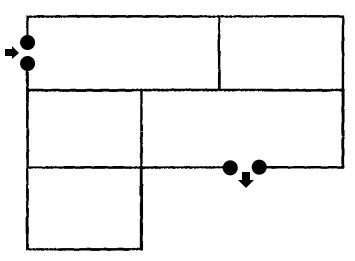
\includegraphics[width=0.7\textwidth]{pic/48.png} }
\end{minipage}

---------------

Автор -- Александр Лазарев
